\def\UrlBreaks{\do\a\do\b\do\c\do\d\do\e\do\f\do\g\do\h\do\i\do\j\do\k\do\l\do\m\do\n\do\o\do\p\do\q\do\r\do\s\do\t\do\u\do\v\do\w\do\x\do\y\do\z\do\A\do\B\do\C\do\D\do\E\do\F\do\G\do\H\do\I\do\J\do\K\do\L\do\M\do\N\do\O\do\P\do\Q\do\R\do\S\do\T\do\U\do\V\do\W\do\X\do\Y\do\Z}
\section{Sequence Diagram}\label{sec:sequenze}
Le tavole seguono UC-03/UC-04, UC-02 e UC-05, descritti nelle
schede della sezione~\ref{sec:template}. I titoli storici conservano il
punto di vista del cliente; la spiegazione adotta quello della concessionaria:
\emph{vendita al cliente} e \emph{acquisto dal cliente}, anche detto
\emph{cessione del cliente}. Non vengono riproposti gateway, unità di lavoro
o strategie della versione precedente.

Ogni tavola distingue l'azione dell'attore, l'handler JavaFX e la chiamata
al servizio, quindi dettaglia le collaborazioni selezionate. I partecipanti
DAO sono le implementazioni PostgreSQL dei contratti già presentati.
Le frecce continue blu sono chiamate sincrone del percorso principale;
quelle rosse evidenziano un'alternativa, i ritorni espliciti sono tratteggiati.
I frammenti \code{alt}/\code{else} sono mutuamente alternativi; \code{loop}
ripete un episodio e \code{ref} rinvia alla collaborazione comune SQ-OB.
Le diciture \guillemotleft{}azione\guillemotright{}, \guillemotleft{}SQL\guillemotright{}, \guillemotleft{}sintesi\guillemotright{} e \guillemotleft{}memoria\guillemotright{} sono descrittive:
non introducono metodi Java. Le note riassumono chiamate effettive omesse
dalle frecce per contenere il numero di linee di vita.

I parametri \code{vehicleId}, \code{clientId}, \code{requestId} e
\code{salesmanId} sono identificativi; \code{Vehicle}, \code{Request},
\code{Model} e \code{BankAccount} sono invece copie in memoria ottenute o
costruite nel flusso. La selezione nella vista non sostituisce una rilettura
transazionale. Le sigle T1--T7 identificano episodi distinti; i nomi delle connessioni
sono locali alla singola tavola. La lettera
\code{c} indica la \code{Connection} effettivamente passata ai DAO.
\code{DatabaseManager} apre la connessione, disabilita autocommit, esegue
la callback e tenta il commit. Su un'\code{Exception} nel corpo o nel commit
tenta rollback, conserva un eventuale errore di rollback come eccezione
soppressa e propaga una \code{RuntimeException}. Il ritorno normale alla
vista segue il commit; errori di apertura, chiusura o comunicazione non
consentono di promettere recupero da qualsiasi guasto o esito sempre conoscibile.

\subsection{Vendita di un veicolo al cliente}
La tavola d'insieme riprende il flusso originale con i collaboratori attuali;
le viste successive approfondiscono transazioni e alternative.
\tavolaautori{sequenza-vendita-insieme}{Vendita al cliente: acconto, autorizzazione e saldo}{fig:sq-vendita-insieme}
\clearpage

La vendita al cliente si articola in sessioni e transazioni separate.
SQ-01a (figura~\ref{fig:sq01a}) copre l'avvio di UC-03: l'aggiornamento
condizionale da \code{SALE} a \code{BLOCKED} precede il calcolo effettivo.
Il prezzo del dialogo è un'anteprima. Il servizio applica la formula con
la base selezionata, automatica o manuale, e fissa totale e acconto del 20\%
nella richiesta \code{SALE}, insieme all'addebito. Come nell'ADR~0001,
la base manuale non è un prezzo finale imposto. Le letture del modello e
degli sconti aprono però connessioni autonome: avvengono durante la callback,
ma fuori dalla transazione di scrittura T1 e senza uno snapshot unico
del listino. Non si attribuisce loro il lock ottenuto sul veicolo.

\begin{figure}[p]
  \centering
  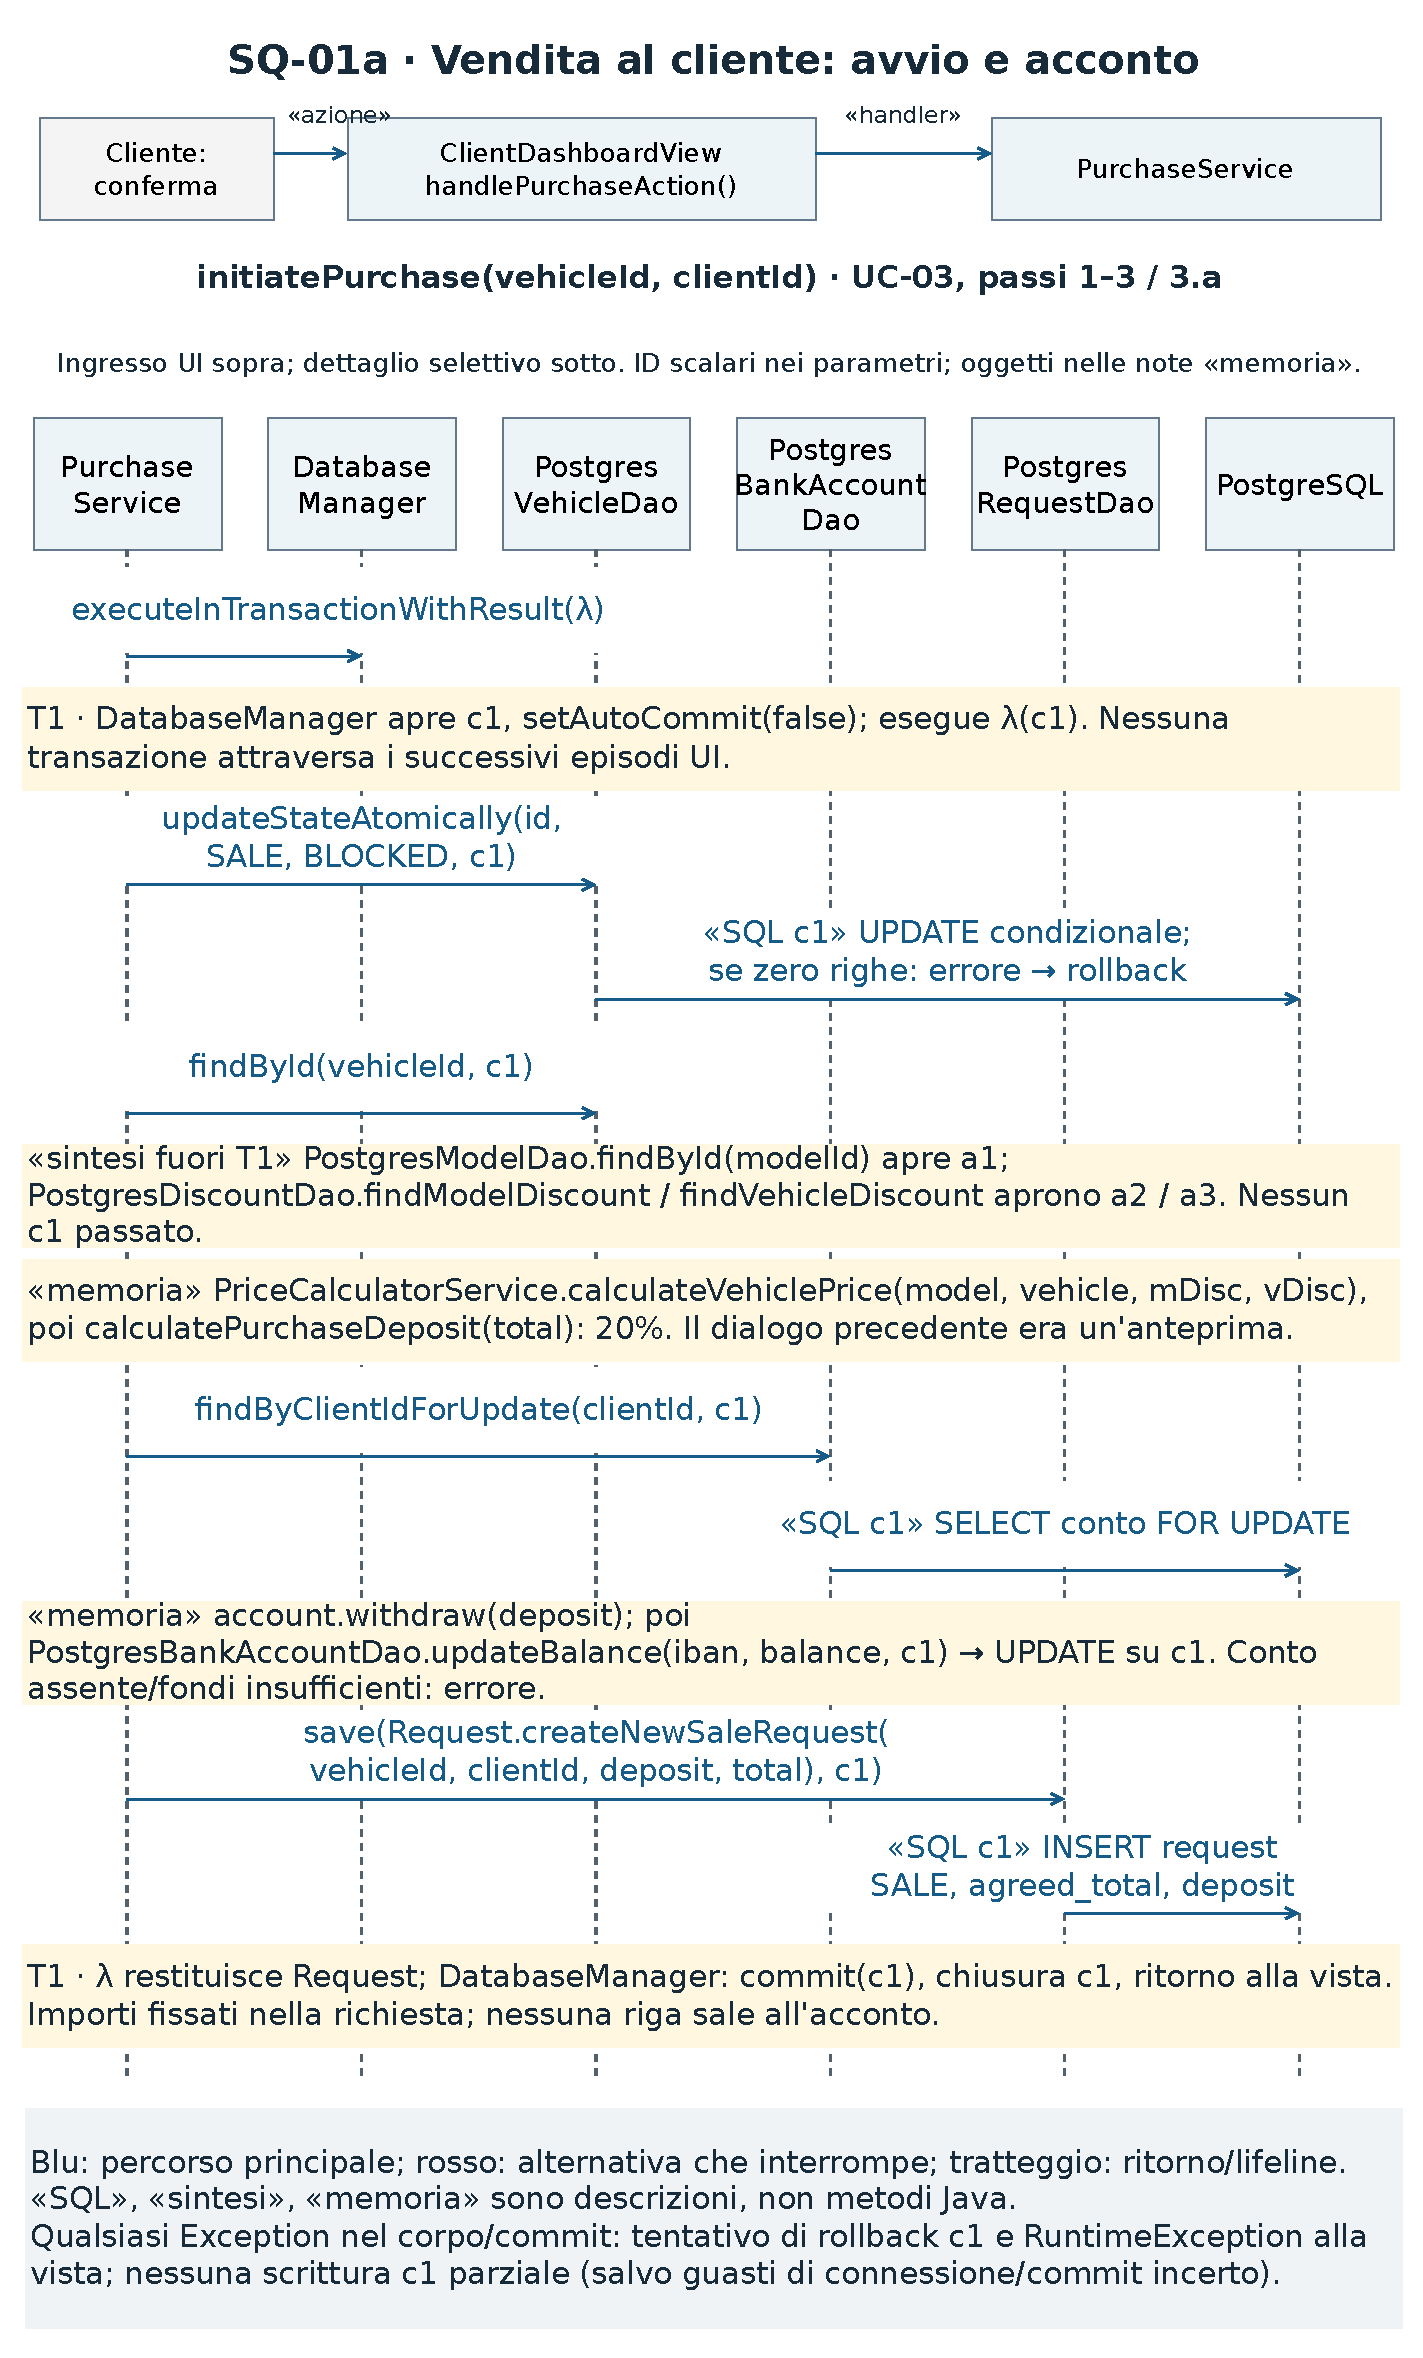
\includegraphics[width=\linewidth,height=.88\textheight,keepaspectratio]{diagrammi/sequenza-vendita-avvio.drawio.pdf}
  \caption{SQ-01a --- Vendita al cliente: avvio, totale concordato e acconto.}\label{fig:sq01a}
\end{figure}
\clearpage

SQ-01b (figura~\ref{fig:sq01b}) rappresenta UC-04: l'approvazione assegna
venditore e scadenza a un mese dalla data corrente, lasciando il veicolo
riservato e il saldo ancora da versare. Il rifiuto restituisce l'intero
acconto, elimina la richiesta e ripristina \code{SALE}. Non crea una penale
né una registrazione nel registro \code{sale}. La richiesta viene riletta
con \texttt{FOR UPDATE}; la lista delle richieste in sospeso è selezionata
dalla UI, mentre il comando non verifica nuovamente che la richiesta non
fosse già approvata. L'autorizzazione di UC-04 è l'esito della richiesta,
non l'abilitazione di un account staff.

SQ-01c (figura~\ref{fig:sq01c}) conclude UC-03. Il servizio rilegge la
richiesta sotto lock, ne controlla tipo, approvazione e scadenza, quindi
addebita \emph{totale concordato meno acconto}, senza ricalcolare il listino.
Il giorno della scadenza è ancora ammesso. Registra l'intero totale come
\code{Sale} di tipo \code{SALE}, elimina la richiesta, porta il veicolo
a \code{SOLD} e notifica sincronicamente l'Observer prima del commit.
Un errore lascia validi gli effetti degli episodi precedenti, come l'acconto
già confermato, e annulla le scritture del solo saldo. I lock coordinano
gli accessi ai record coinvolti; i servizi di saldo ed esito ricevono ID,
senza un'identità del chiamante con cui provare un controllo generale dei permessi.

\begin{figure}[p]
  \centering
  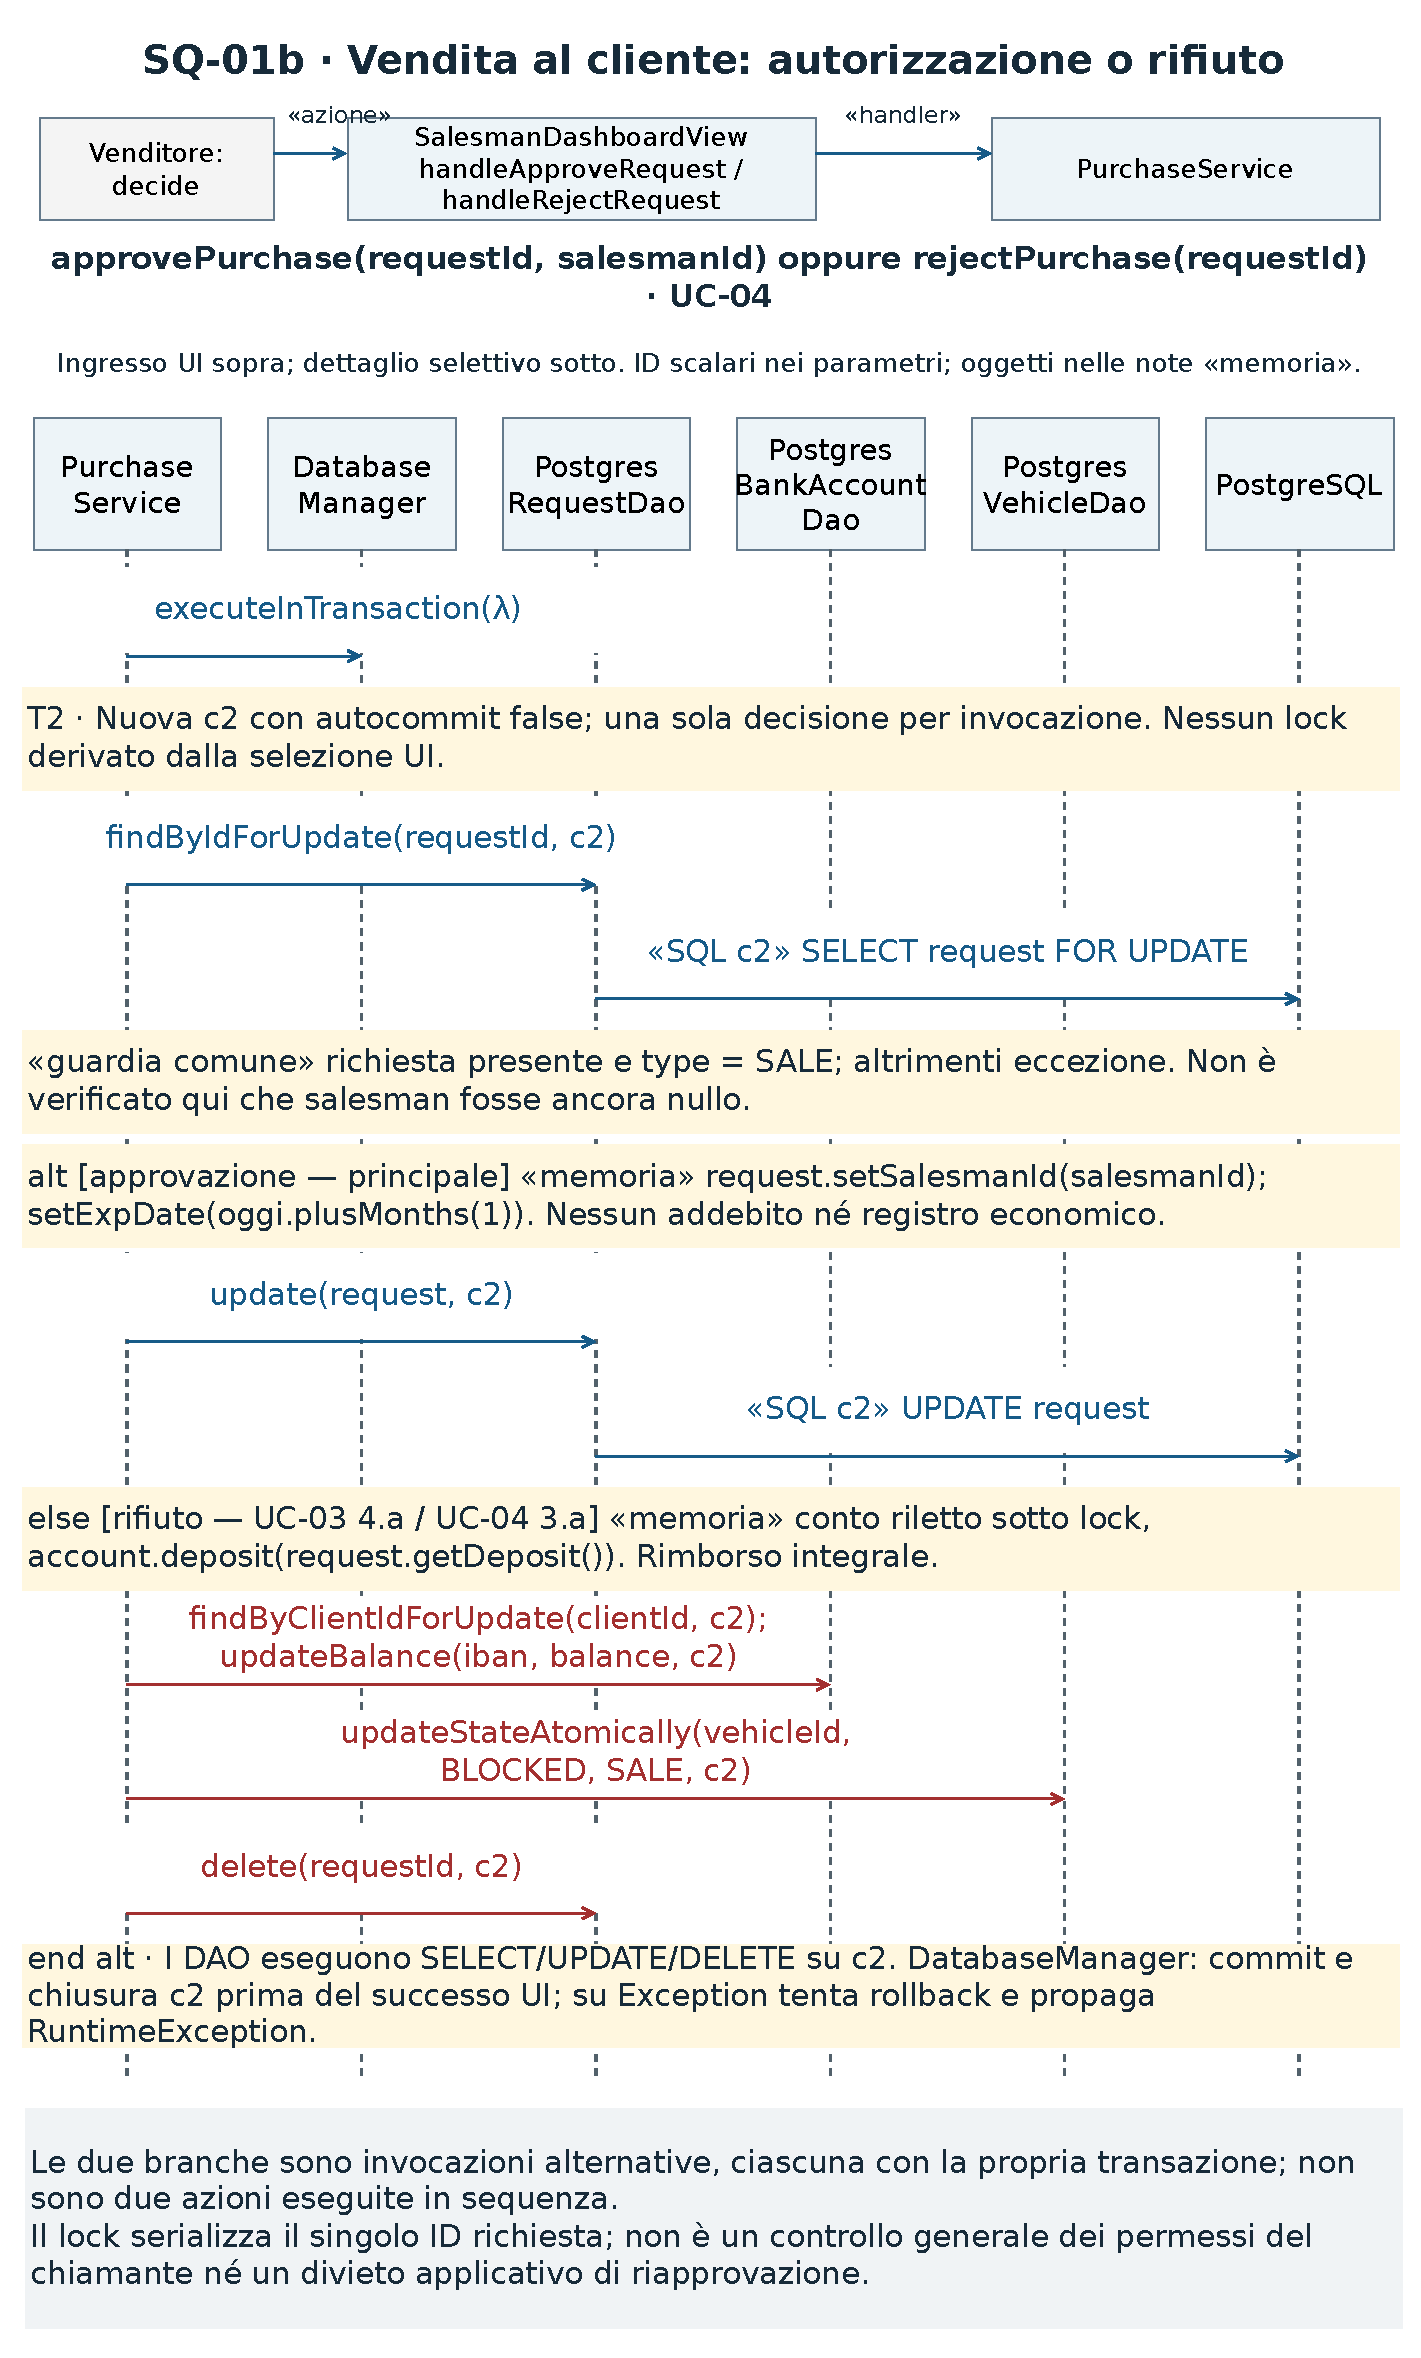
\includegraphics[width=\linewidth,height=.88\textheight,keepaspectratio]{diagrammi/sequenza-vendita-esito.drawio.pdf}
  \caption{SQ-01b --- UC-04: approvazione oppure rifiuto con rimborso.}\label{fig:sq01b}
\end{figure}
\begin{figure}[p]
  \centering
  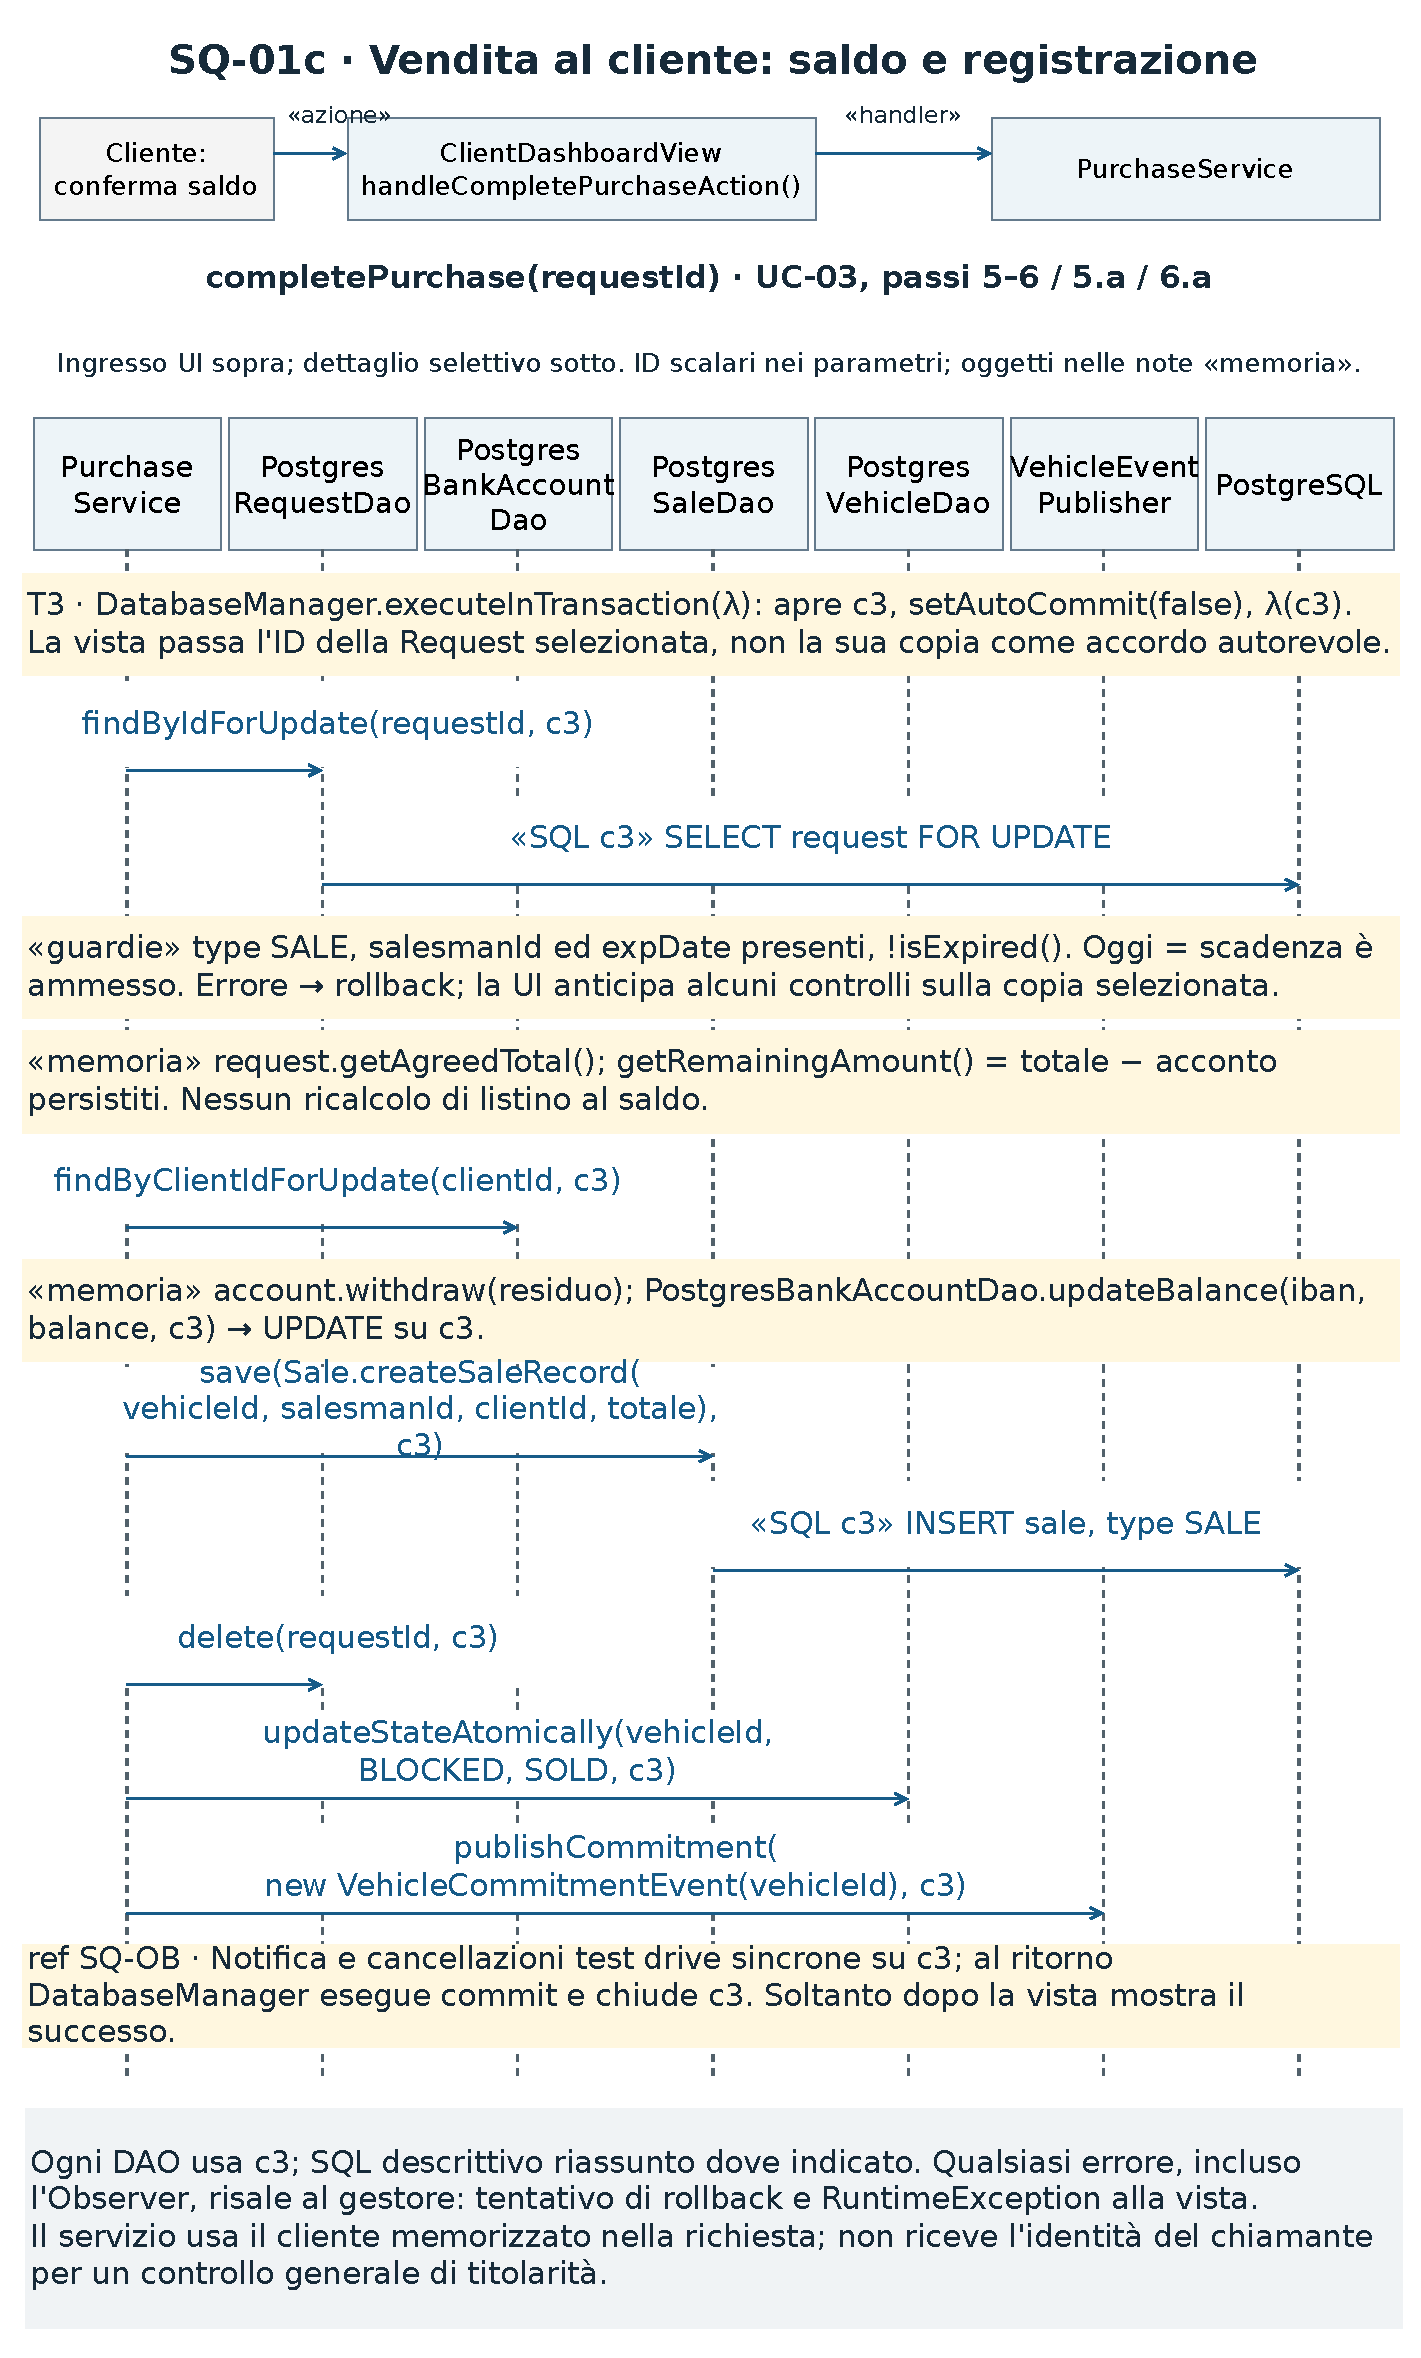
\includegraphics[width=\linewidth,height=.88\textheight,keepaspectratio]{diagrammi/sequenza-vendita-saldo.drawio.pdf}
  \caption{SQ-01c --- Saldo sul totale persistito e registrazione della vendita al cliente.}\label{fig:sq01c}
\end{figure}
\clearpage

SQ-01d (figura~\ref{fig:sq01d}) copre l'alternativa UC-03 6.b.
Il costruttore della dashboard cliente programma il controllo con
\code{Platform.runLater}: non è un processo periodico e il solo decorso
del tempo non esegue movimenti. Una lettura autonoma raccoglie i candidati;
ciascuno è poi riletto e valutato in una transazione propria. Per una
richiesta approvata con data strettamente precedente a oggi, il servizio
trattiene il 20\% dell'acconto, arrotondato ai centesimi, restituisce il resto,
registra \code{PENALTY}, elimina la richiesta e libera il veicolo.
La penale non è il 20\% del totale. Un candidato non più pertinente non
produce effetti; se un candidato fallisce, quelli già confermati restano
trattati. L'errore risale alla vista, che in questo controllo scrive un
avviso su stderr; i messaggi all'utente sono mostrati solo al ritorno
normale della lista. Non si produce una notifica Observer.

\begin{figure}[p]
  \centering
  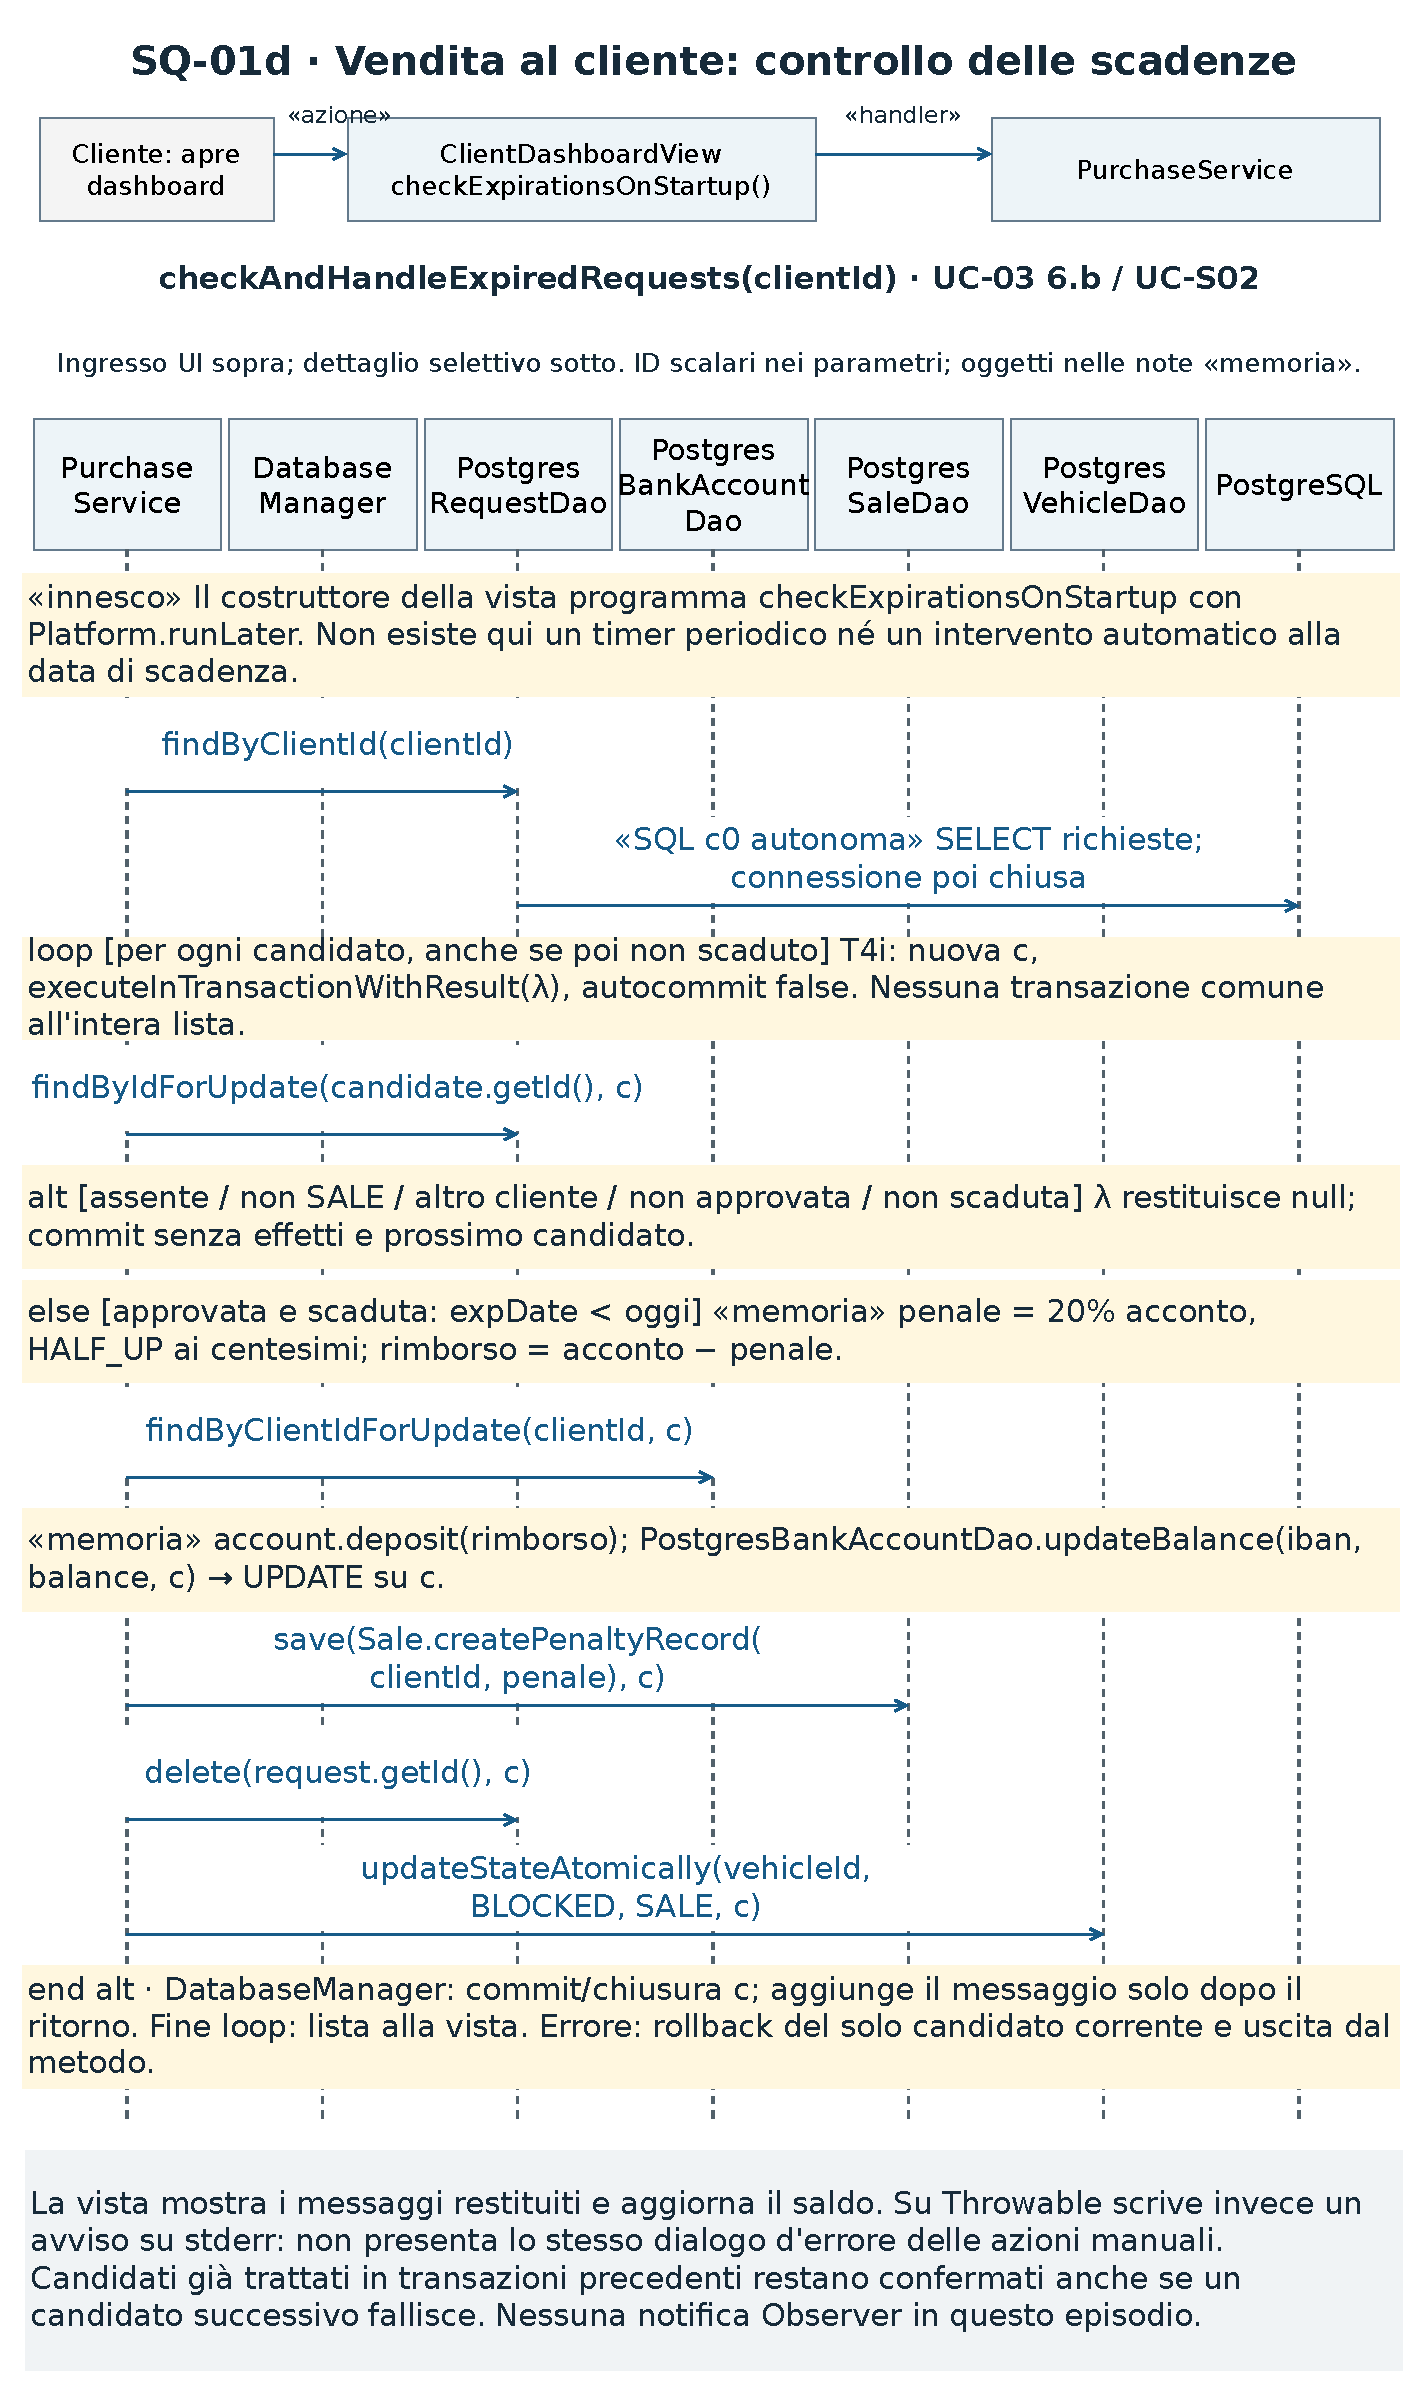
\includegraphics[width=\linewidth,height=.88\textheight,keepaspectratio]{diagrammi/sequenza-vendita-scadenza.drawio.pdf}
  \caption{SQ-01d --- Scadenze controllate all'apertura della dashboard, una transazione per candidato.}\label{fig:sq01d}
\end{figure}
\clearpage

\subsection{Prenotazione di un noleggio}
La tavola d'insieme riprende il flusso originale con i collaboratori attuali;
le viste successive approfondiscono transazioni e alternative.
\tavolaautori{sequenza-noleggio-insieme}{Noleggio: prenotazione e impegno commerciale}{fig:sq-noleggio-insieme}
\clearpage

SQ-02 (figura~\ref{fig:sq02}) realizza UC-02. Il preventivo del dialogo
è calcolato in una chiamata distinta e non congela un accordo.
Alla conferma, il servizio rifiuta date passate o invertite, blocca il
veicolo con \texttt{FOR UPDATE}, richiede \code{RENT} e blocca l'identità
cliente con \texttt{FOR NO KEY UPDATE}. Rilegge quindi la disponibilità sul
periodo incluso, ricalcola il costo e addebita il 100\% sotto lock del conto.
Gli overload PostgreSQL delle letture di modello e sconti usati qui
ricevono la stessa connessione: ciò non equivale a uno snapshot globale
immutabile né a un lock dell'intero listino. Lo stato rimane \code{RENT}.

Il controllo applicativo dei periodi è affiancato dal vincolo SQL
\code{EXCLUDE} sui noleggi dello stesso veicolo. Dopo il salvataggio,
la collaborazione SQ-OB (figura~\ref{fig:sqob}) cancella \emph{tutti} i
test drive futuri del veicolo, anche esterni al periodo noleggiato:
è la priorità commerciale condivisa con il saldo della vendita al cliente.
Il publisher chiama direttamente l'Observer sullo stesso thread e sulla
stessa connessione, prima del commit. Un errore della cancellazione risale
al gestore e impedisce di confermare addebito e prenotazione separatamente.
Non vi sono coda, outbox o consegna asincrona. Il servizio di noleggio
riespone le cause applicative riconosciute, mentre gli altri errori
rimangono avvolti; la vista presenta il fallimento. Non si estende questa
garanzia ad altre operazioni o a qualsiasi protocollo concorrente.

\begin{figure}[p]
  \centering
  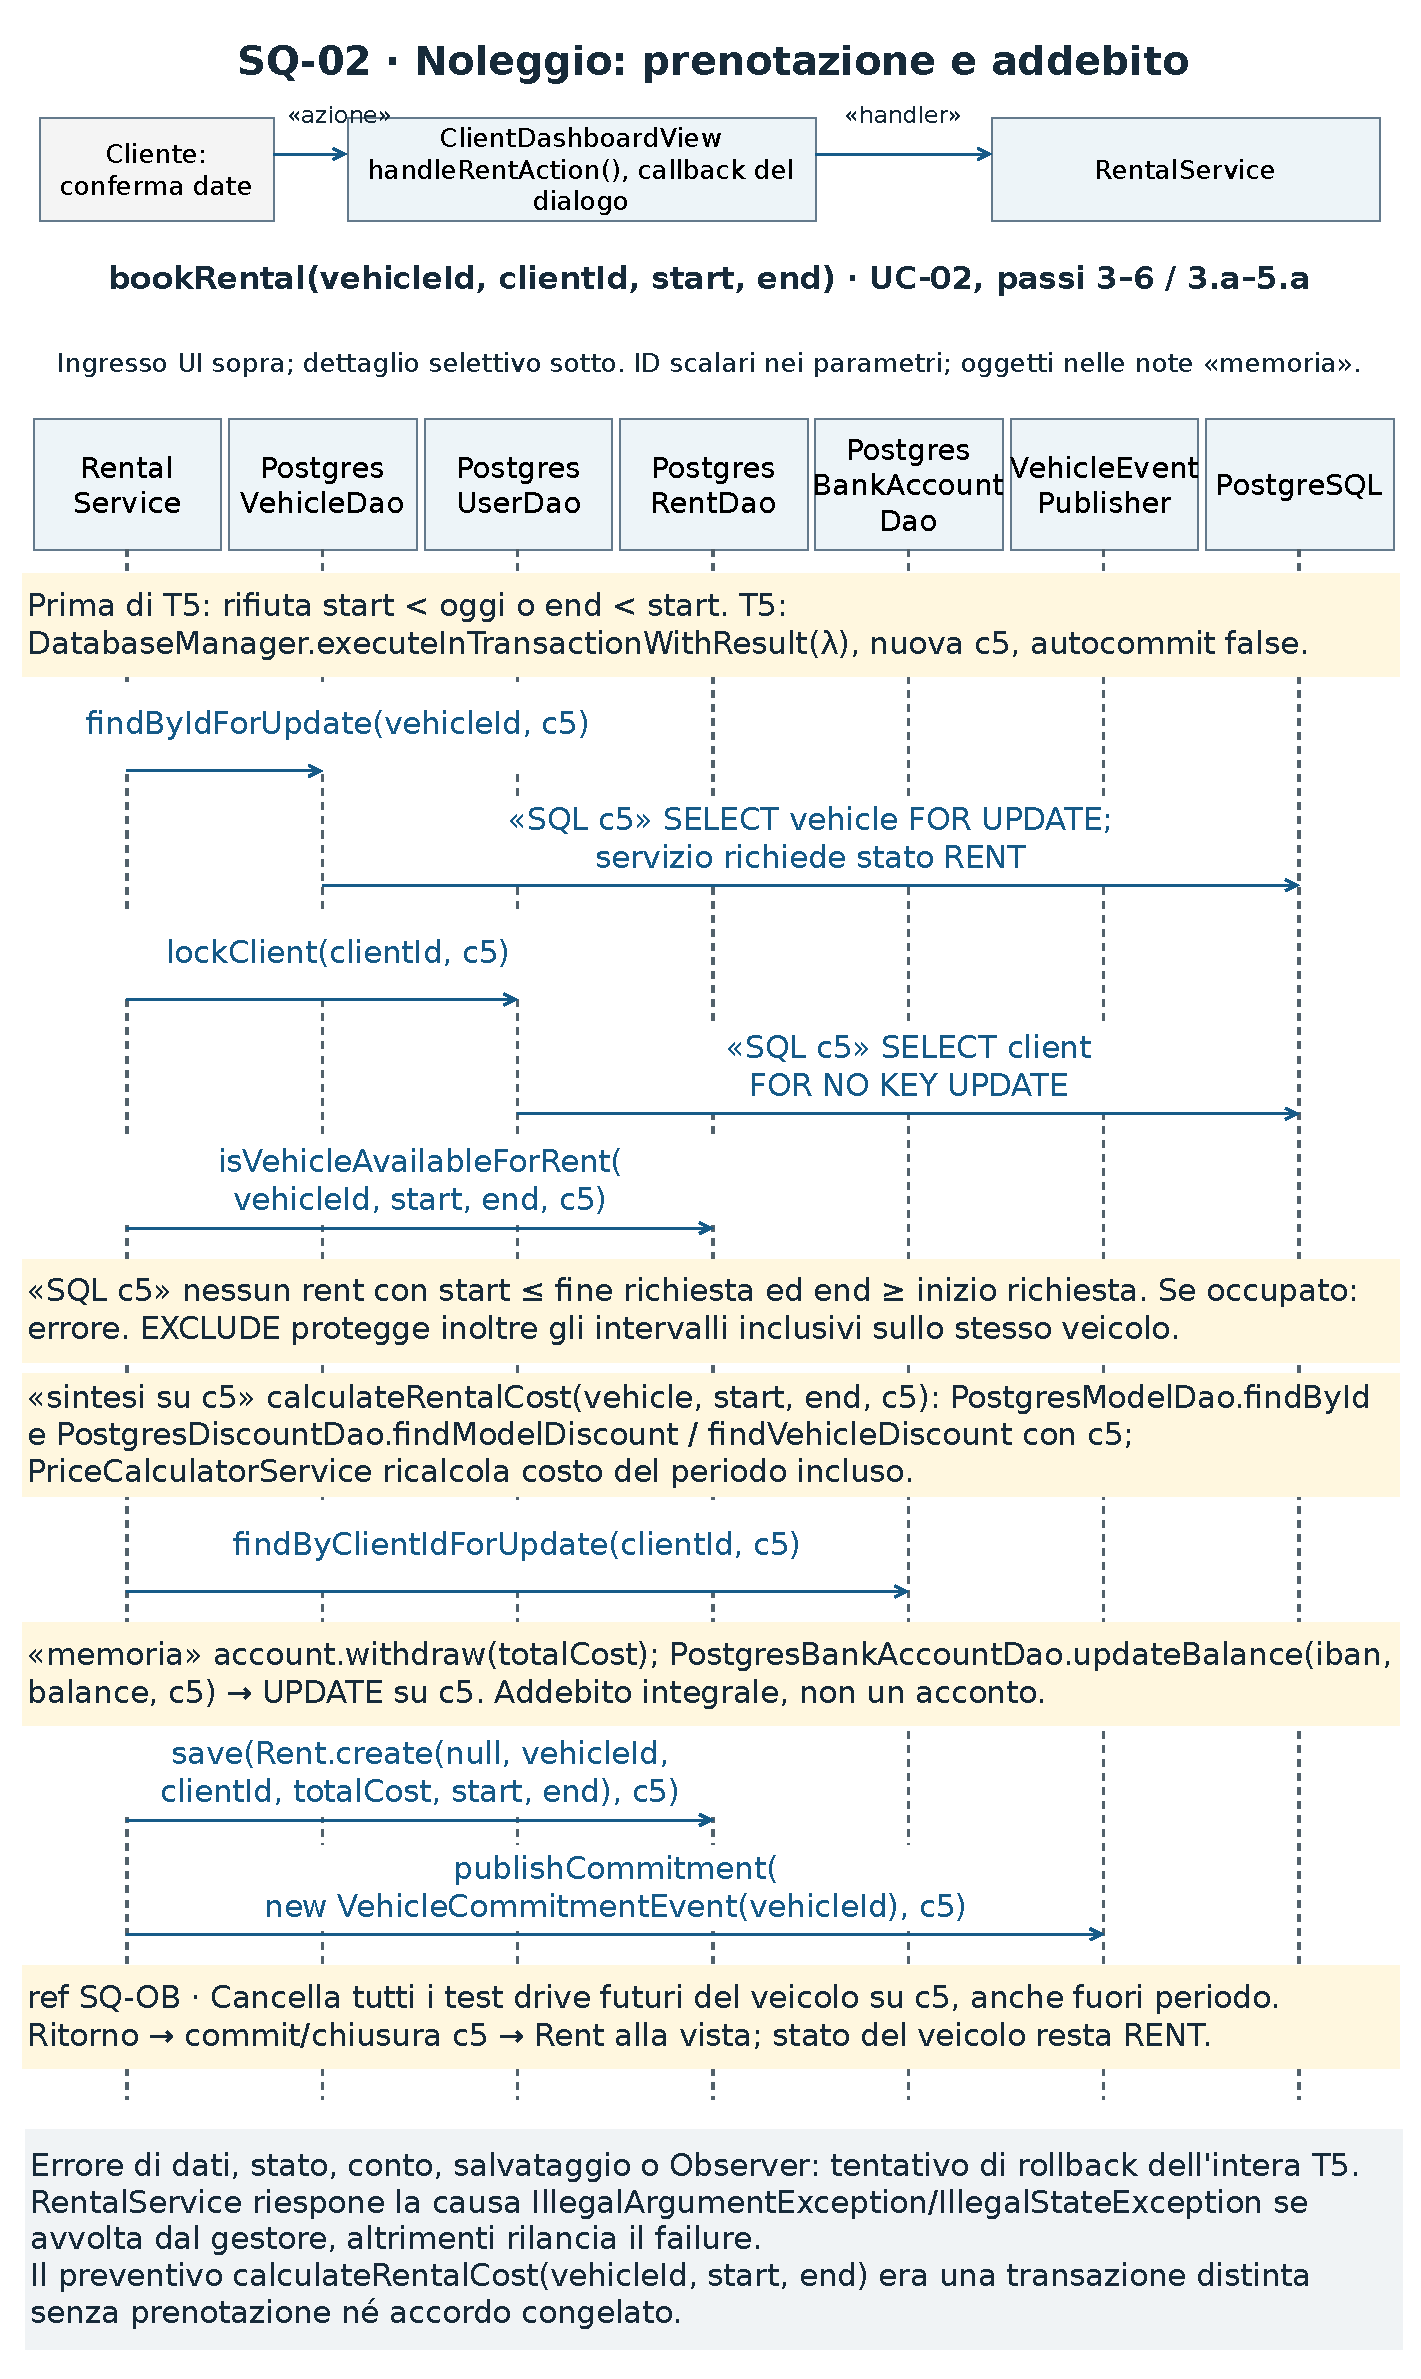
\includegraphics[width=\linewidth,height=.88\textheight,keepaspectratio]{diagrammi/sequenza-noleggio.drawio.pdf}
  \caption{SQ-02 --- Noleggio: disponibilità, costo ricalcolato e addebito integrale.}\label{fig:sq02}
\end{figure}
\begin{figure}[p]
  \centering
  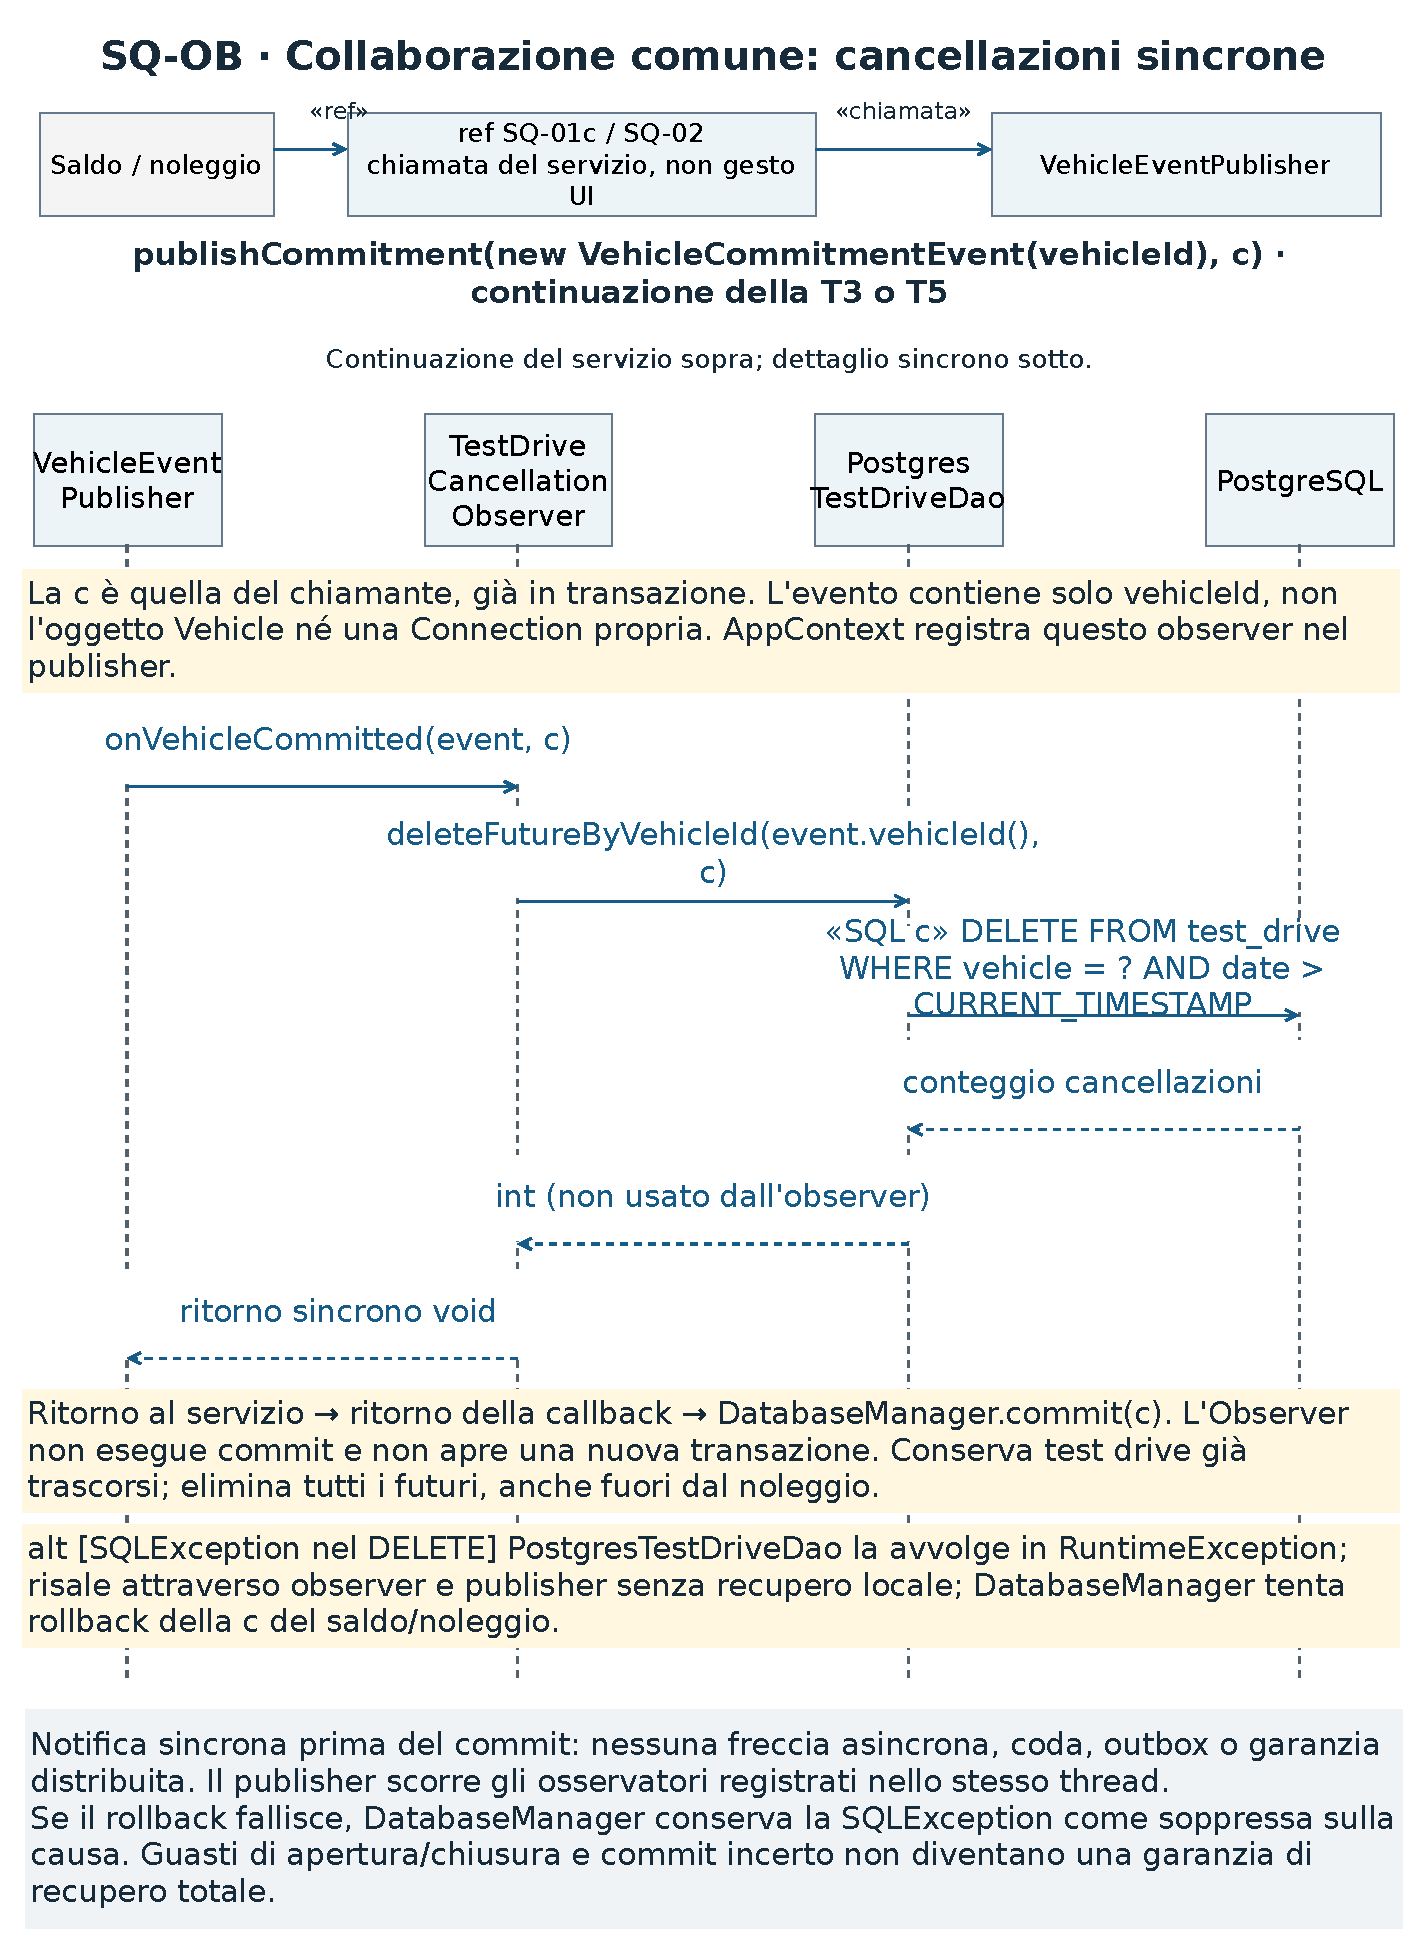
\includegraphics[width=\linewidth,height=.88\textheight,keepaspectratio]{diagrammi/sequenza-observer.drawio.pdf}
  \caption{SQ-OB --- Cancellazioni Observer condivise da SQ-01c e SQ-02, sincrone sulla connessione del chiamante.}\label{fig:sqob}
\end{figure}
\clearpage

\subsection{Acquisto di un veicolo dal cliente}
La tavola d'insieme riprende il flusso originale con i collaboratori attuali;
le viste successive approfondiscono transazioni e alternative.
\tavolaautori{sequenza-cessione-insieme}{Acquisto dal cliente: proposta ed esito}{fig:sq-cessione-insieme}
\clearpage

L'acquisto dal cliente di UC-05 ha due episodi distinti.
SQ-03a (figura~\ref{fig:sq03a}) registra la proposta e non effettua
pagamenti. Se il VIN è noto, il veicolo deve essere \code{SOLD},
l'ultima vendita al cliente deve attribuirlo al proponente e non devono
esistere richieste aperte; modello e anno devono coincidere. Il lock
\texttt{FOR UPDATE} riguarda una riga esistente, non un VIN assente.
Per un VIN nuovo viene creato il veicolo; in entrambi i casi lo stato
è \code{WAITING}. Il servizio ricalcola la stima e la salva in
\code{Request.deposit}, di tipo \code{PURCHASE}, con
\code{agreed\_total} nullo. Le letture autonome del modello e dello
sconto modello non appartengono a T6. La stima persistita, non il
preventivo facoltativo della UI, fissa l'importo dell'eventuale accettazione.

SQ-03b (figura~\ref{fig:sq03b}) rilegge e blocca richiesta e veicolo,
richiedendo rispettivamente \code{PURCHASE} e \code{WAITING}.
L'accettazione richiede il venditore, accredita la stima memorizzata,
registra \code{Sale} di tipo \code{PURCHASE}, porta il veicolo a
\code{SALE} ed elimina la richiesta nella stessa transazione.
L'importo è non negativo ed esprime un esborso della concessionaria;
non è un acconto seguito da un saldo. Il rifiuto non movimenta il conto:
elimina la richiesta e, secondo le operazioni associate, ripristina
\code{SOLD} oppure elimina il veicolo senza storico. La presenza di
storico non sostituisce il controllo dell'ultima vendita al proponente.
Non interviene l'Observer. Un errore annulla l'esito corrente.

Un limite applicativo riguarda gli importi pari a zero: le richieste e
lo schema li ammettono, mentre il conto richiede movimenti strettamente
positivi. Un accredito o addebito zero nei percorsi rappresentati fallisce
e provoca rollback. Il limite del movimento non equivale quindi a un
divieto di conservare valori zero nelle richieste e nel registro.

\begin{figure}[p]
  \centering
  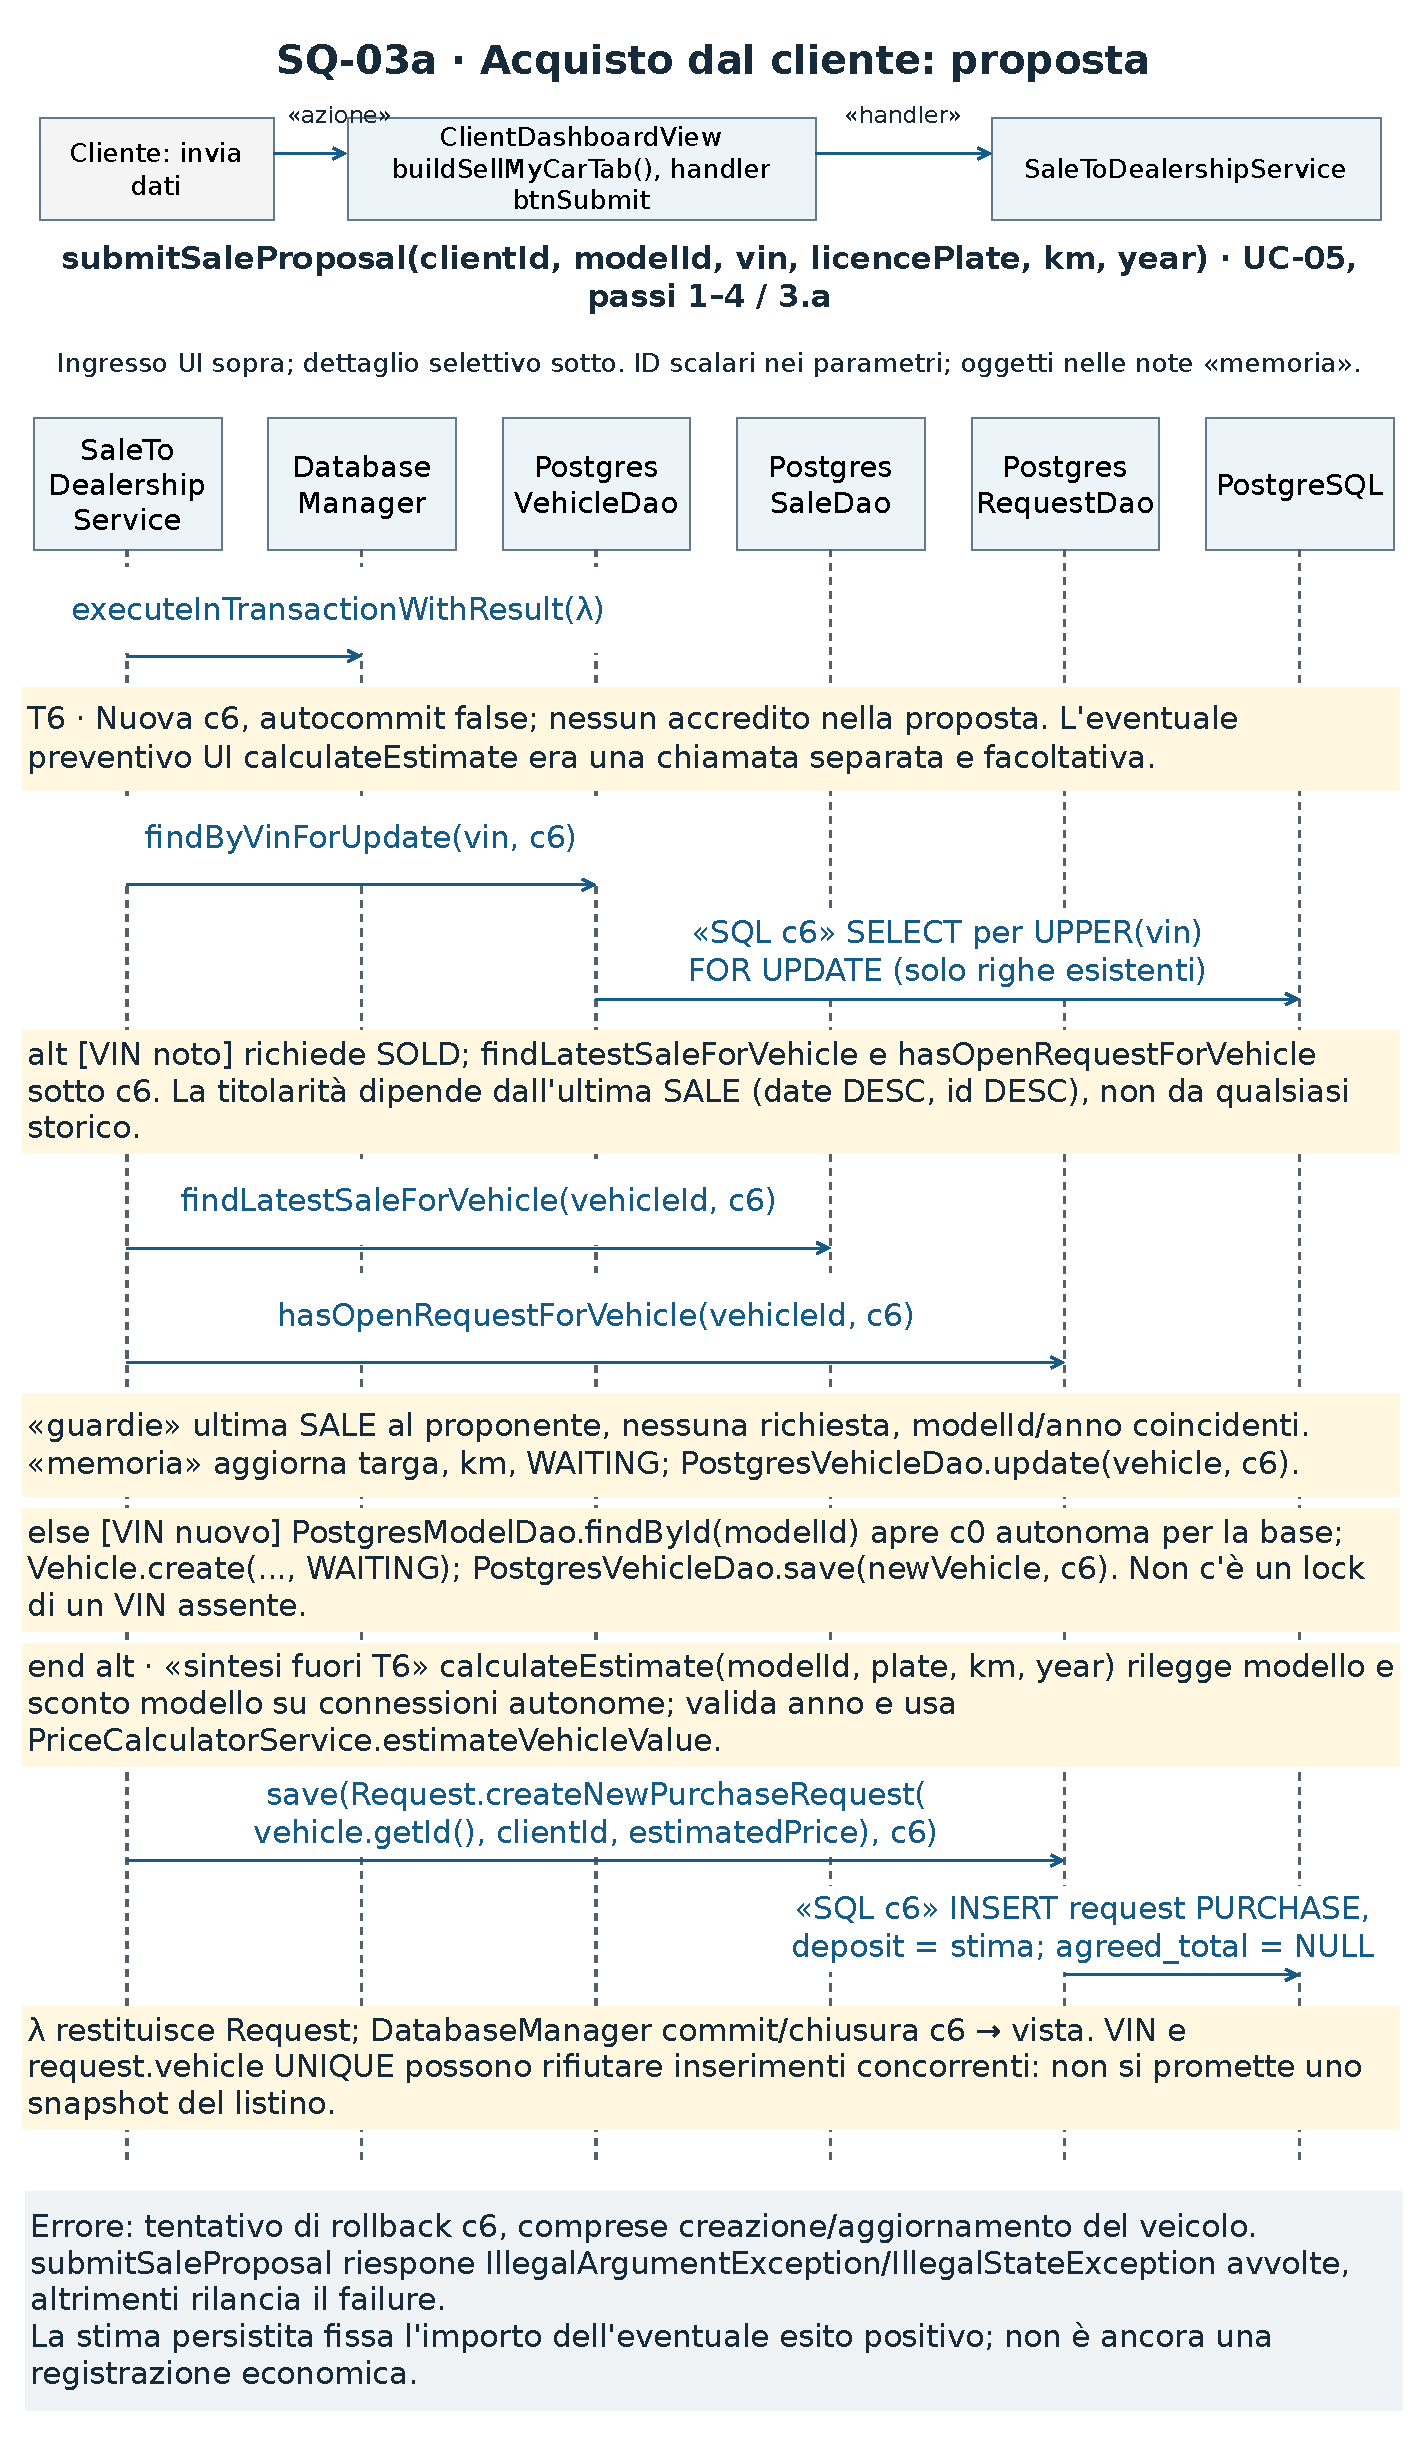
\includegraphics[width=\linewidth,height=.88\textheight,keepaspectratio]{diagrammi/sequenza-cessione-proposta.drawio.pdf}
  \caption{SQ-03a --- Proposta di cessione: veicolo in attesa e stima persistita, senza pagamento.}\label{fig:sq03a}
\end{figure}
\begin{figure}[p]
  \centering
  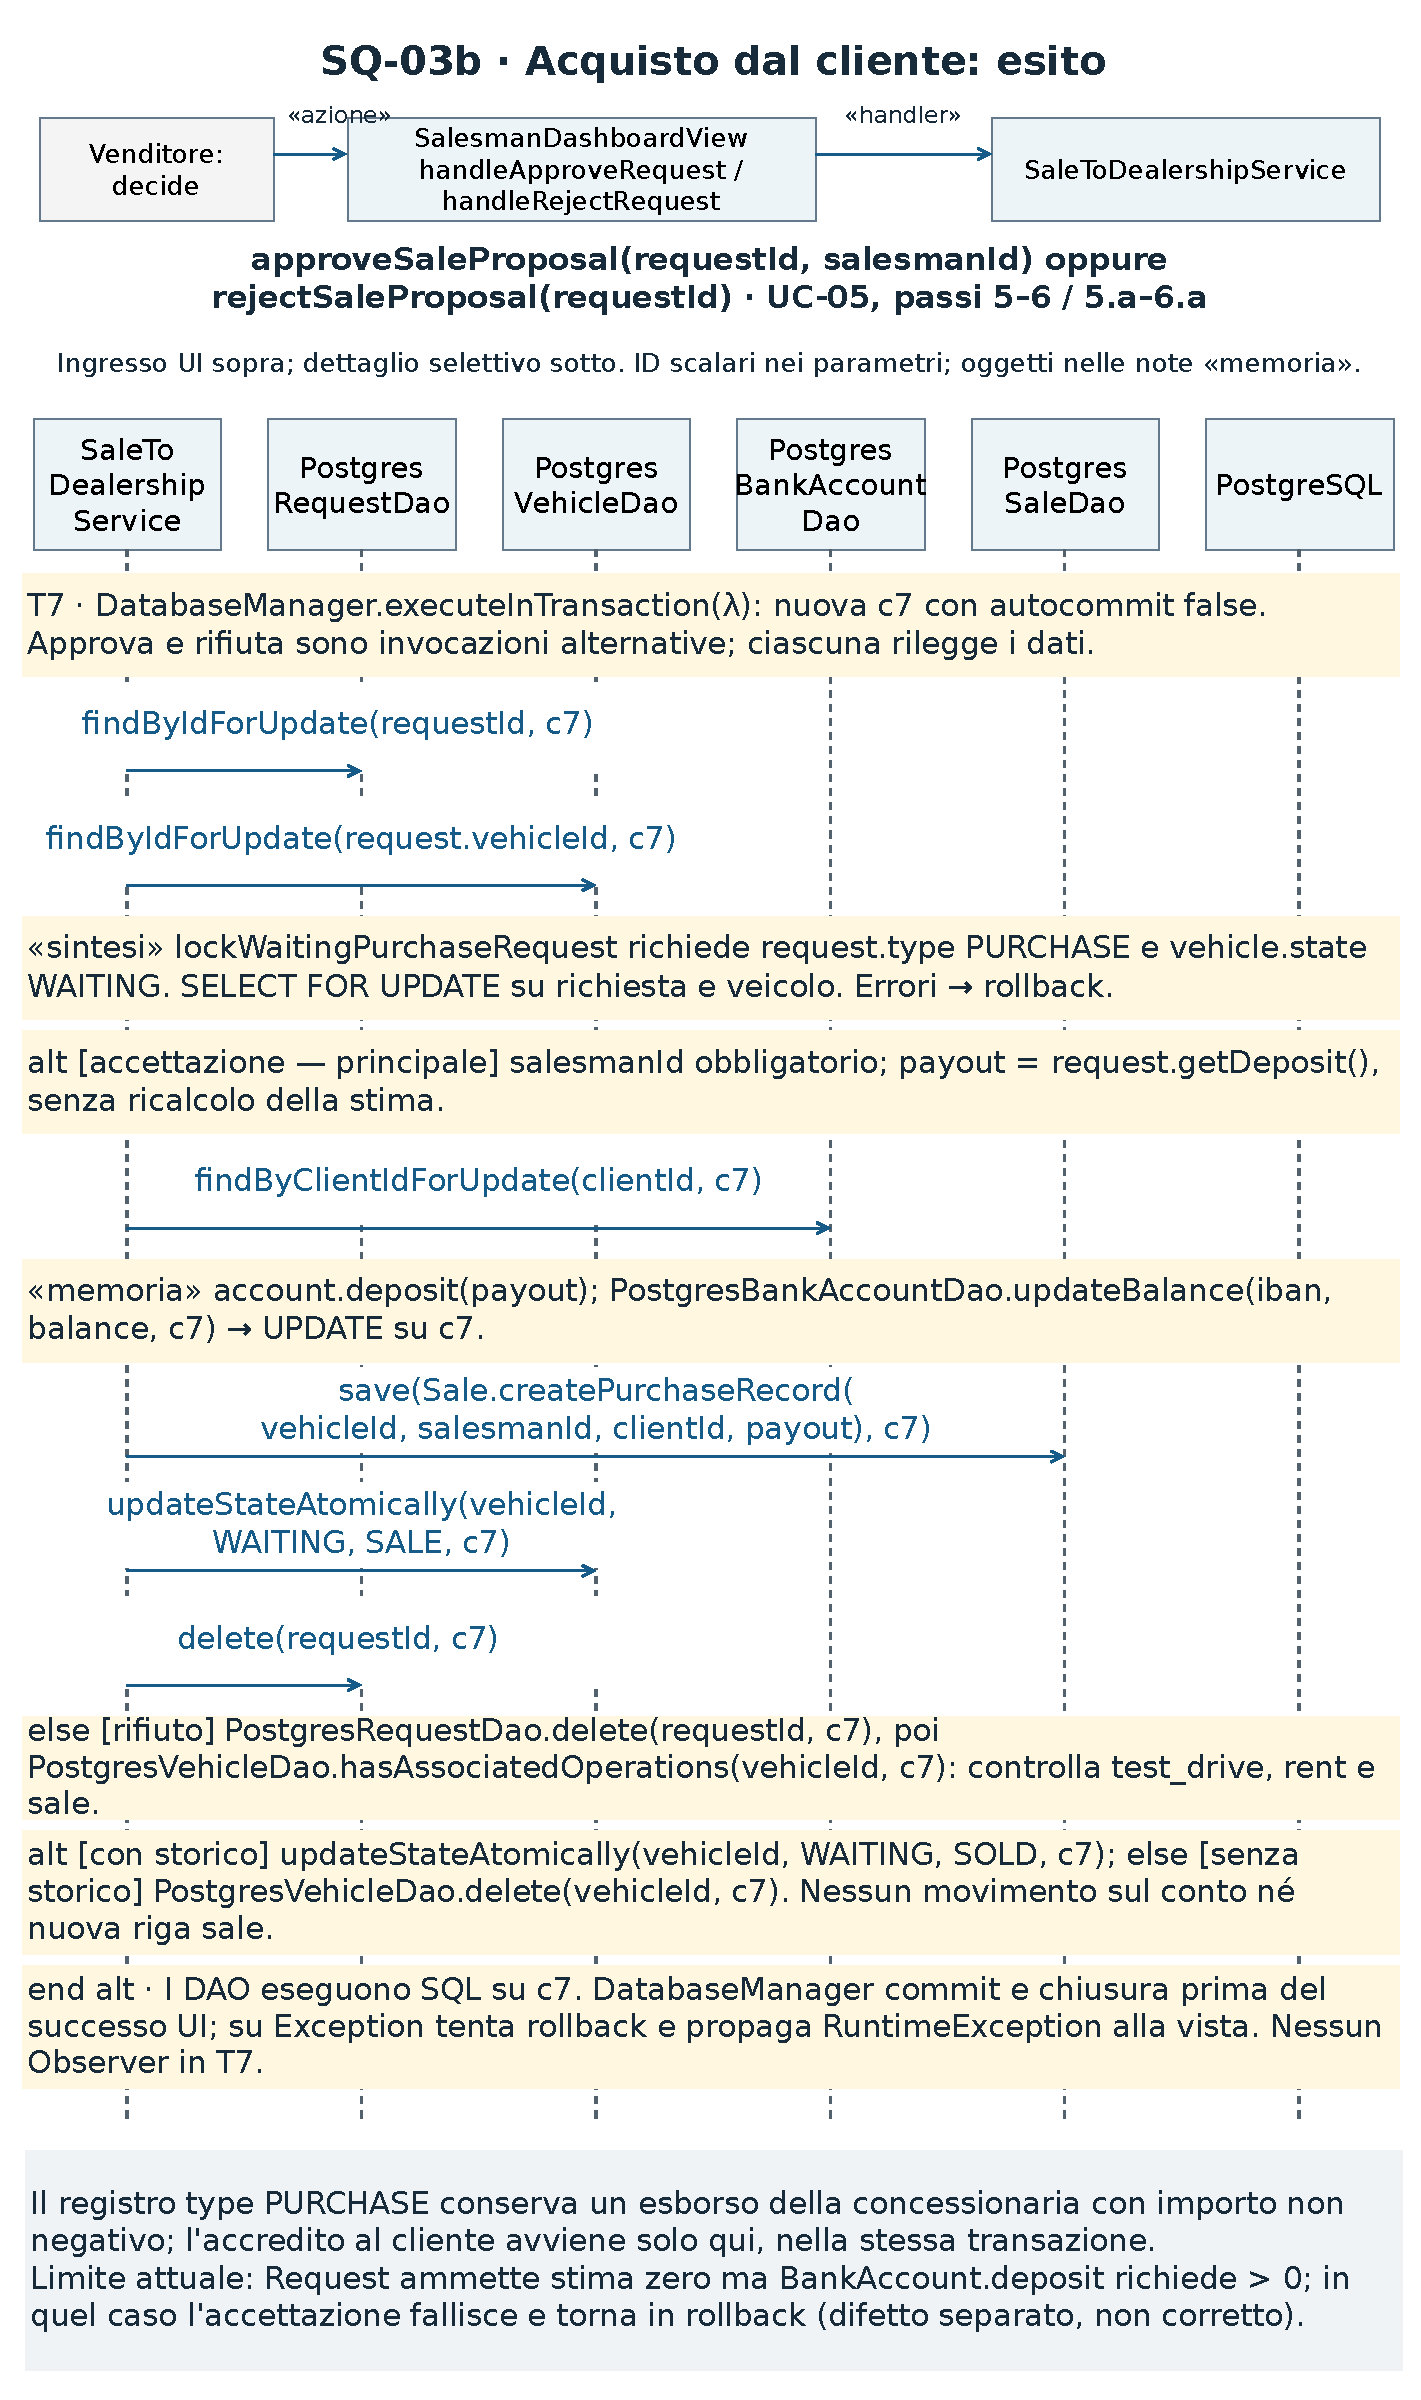
\includegraphics[width=\linewidth,height=.88\textheight,keepaspectratio]{diagrammi/sequenza-cessione-esito.drawio.pdf}
  \caption{SQ-03b --- Acquisto dal cliente: accettazione economica oppure rifiuto con conservazione dello storico.}\label{fig:sq03b}
\end{figure}
\clearpage
